\begin{frame}
    \frametitle{\problemtitle}
    \begin{itemize}
        \item<+-> \textbf{Problem:} Given $n$ concentric circles,
        	find the maximal number of points on these circles
        	such that the distance between any two points is at least $e$.
        \item<+-> \textbf{Observation:} Because $r_{i+1}-r_i \geq e$,
        	each circle can be considered separately.
    \end{itemize}
    \vspace{-1.5em}

    \begin{columns}
    \begin{column}{0.0\textwidth}
    \end{column}
    \begin{column}{0.7\textwidth}
    \begin{itemize}
        \item<+-> The number of points on circle $i$ is
        	\[\left\lfloor\frac{2\pi}{2\arcsin(\frac{e}{2r_i})}\right\rfloor.\]
        \item<+-> Edge case: if $2r_i < e$, the number of points is $1$.

    	\item<+-> Beware floating point issues!
    	\begin{itemize}
    		\item<+-> Add $0.5 \cdot 10^{-6}$ to every radius.
    	\end{itemize}
    \end{itemize}
    \end{column}
    \begin{column}{0.3\textwidth}
      \begin{center}
        \onslide<3->{
        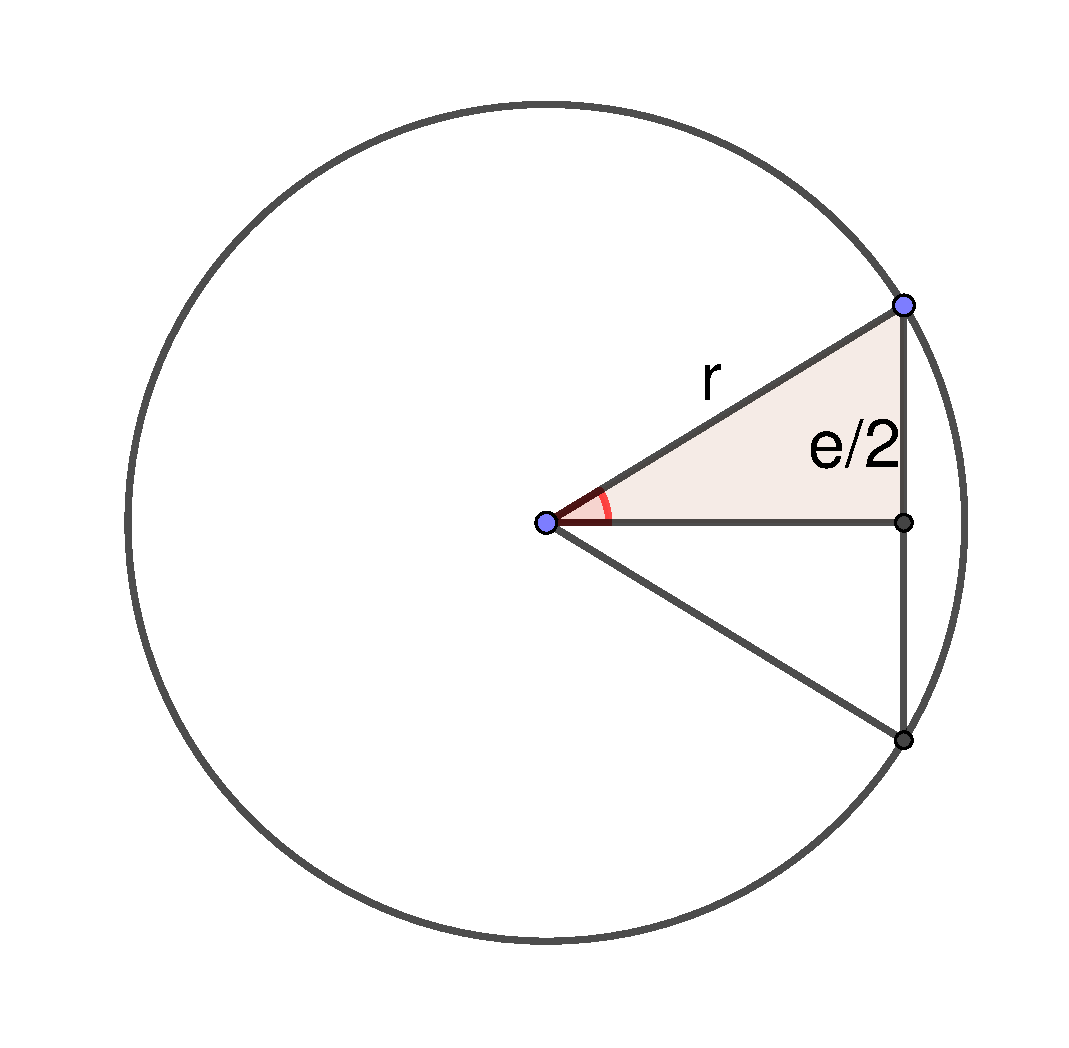
\includegraphics[width=\textwidth]{jets.pdf}
        }
      \end{center}
    \end{column}
    \end{columns}
    \solvestats
\end{frame}
